\author[Felix Hekhorn]{}
\institute{University of Milan}

\newcommand{\mmsbar}{{\overline{\rm {MS}}}}
\newcommand{\msbar}{$\mmsbar$}
\definecolor{UniSec6}{RGB}{50,110,30}
\providecommand{\iRef}[1]{{\tiny\color{UniSec6} $[$#1$]$}}

\subsection{PDF Positivity (TH)}

\begin{frame}{Positivity - Theory}
A. Candido, S. Forte, \underline{F. Hekhorn} \iRef{JHEP 11 (2020) 129}\\
{\bf Can \msbar{} parton distributions be negative?}\\
{\large \hfill \bf No!}

DIS: $F = \sum_j c_j \otimes f_j$

LO: Structure Function = PDF \checkmark

gluon@NLO:\\
\newcolumntype{e}{>{\centering\arraybackslash} m{.5\linewidth} }
\begin{tabular}{ee}
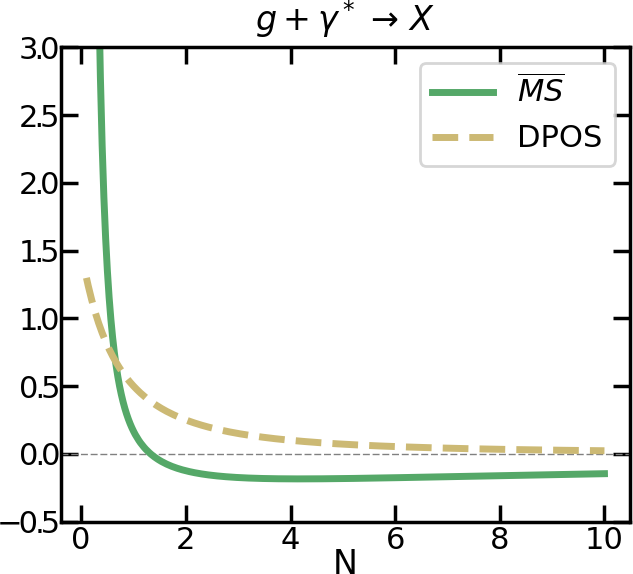
\includegraphics[height=4cm]{felix_positivity/disg.png}
&
\begin{itemize}
\item $c_g^{(1), bare}(z,Q^2,\epsilon) > 0$ \checkmark
\item $c_g^{(1), \mmsbar}(z) < 0$ for $z \to 1$
\item $c_g^{(1), \rm{DPOS}}(z) > 0$ \checkmark
\item $c_g^{(1), \rm{DIS}}(z) = 0$ \checkmark
\end{itemize}
\end{tabular}

\end{frame}

\begin{frame}{Positivity - Theory}
\begin{center}
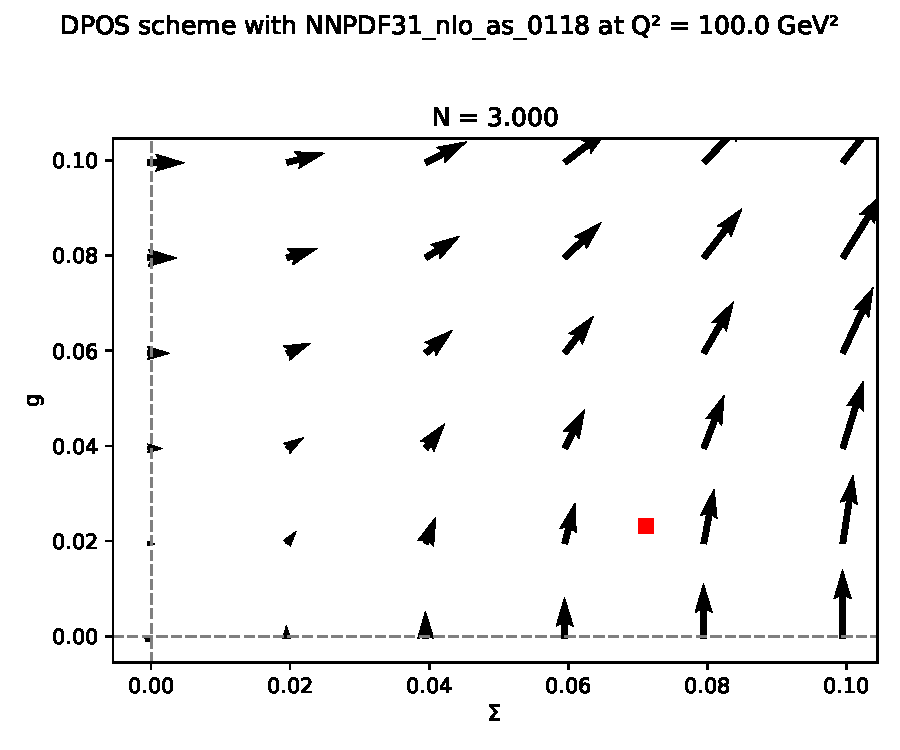
\includegraphics[height=5cm]{felix_positivity/quiver2-NNPDF31_nlo_as_0118-100_0-tiny-8.pdf}
\end{center}
\vspace{-2pt}
DPOS $\to$ \msbar: for $z < 1$ use perturbativity, for $z\to 1$ use \textit{exact} transformation $\Rightarrow \mmsbar > 0$\\
To obtain a physical xs/PDF is positivity {\bf sufficient?} no!\\
\hspace{149pt} or even {\bf necessary?} no!\\
$\Rightarrow$ but we can prove they \textit{are} positive and so it adds a cut in PDF space!
\end{frame}

